% Compile with:
% latexmk -pdf -pvc -interaction=nonstopmode
%\documentclass[aspectratio=169,10pt,draft]{beamer}
\documentclass[aspectratio=169, 10pt]{beamer}
\usetheme{UniBern}
\title{Adaptation Mechanisms Of Zebrafish Respiratory Organ To Endurance Training}
\author{David Haberthür \and
	Dea Aaldijk \and
	Matthias Messerli \and
	Fluri A.\ M.\ Wieland \and
	Oleksiy Khoma \and
	Helena Röss \and
	Ruslan Hlushchuk}
\institute{Institute of Anatomy\\University of Bern\\Switzerland}
\date{June 5, 2019 | \href{https://www.bruker.com/events/micro-ct-users-meeting.html}{Bruker micro-CT Users Meeting 2019}}

%\includeonlyframes{current}
%then....
%\begin{frame}[label=current]
%\end{frame}

\usepackage[english]{babel}
\usepackage{microtype}
\usepackage[backend=biber,
	style=numeric,
	url=false,
	isbn=true,
	maxbibnames=1,
	sorting=none,
	backref=true]{biblatex}
	\addbibresource{../../Documents/library.bib}
\usepackage{graphicx}
\usepackage{tikz}
	%\usetikzlibrary{external}
	%\tikzexternalize[prefix=tikz/]
\usepackage{pgfplots}
	\pgfplotsset{compat=newest}
\usepackage[detect-all=true, range-phrase=--, range-units=single, binary-units=true]{siunitx}
\usepackage[absolute,overlay]{textpos} %for the \source{} command
\usepackage{gitinfo2}
\usepackage[version=4]{mhchem}
\usepackage{xspace}
\usepackage{ccicons}
\usepackage{multimedia}
\usepackage{animate}
\usepackage{listings}
	\lstset{
		frame=shadowbox,
		rulesepcolor=\color{ubRed},
		basicstyle=\scriptsize
		}
\usepackage{fontawesome5}
\usepackage[eulergreek]{sansmath} % change tikz font to slide font, courtesy of https://tex.stackexchange.com/a/33329/828
	\pgfplotsset{
		tick label style = {font=\sansmath\sffamily},
		every axis label = {font=\sansmath\sffamily},
		legend style = {font=\sansmath\sffamily},
		label style = {font=\sansmath\sffamily}
		}
\usepackage{media9}		

% Some often used abbreviations
\newcommand{\imsize}{\linewidth} % set global image width
\newcommand{\everyframe}{12} % use only every nth frame for the movies
\newlength\imagewidth % needed for scalebars
\newlength\imagescale % needed for scalebars
\newcommand{\uct}{\si{\micro}CT\xspace} % make our life easier

% Easily fill a frame with the whole image.
% Based on http://tex.stackexchange.com/a/334758/828,
\newcommand{\fullframeimage}[1]{%
	\begin{tikzpicture}[remember picture,overlay]%
		\node[xshift=0,yshift=0] at (current page.center){%
			\includegraphics[width=\paperwidth]{#1}};%		
	\end{tikzpicture}%
}

% Acknowledge images just below them
% Based on https://tex.stackexchange.com/a/206925/828
%\newcommand{\source}[2]{\par\hfill\tiny \href{http://#1}{#1} #2}
% Based on https://tex.stackexchange.com/a/282637
\newcommand{\source}[2]{%
	\raisebox{-1ex}{\makebox[0pt][r]{\tiny \href{http://#1}{#1} #2}}
}

% Define us our custom footer
\defbeamertemplate{footline}{unibe}{%
	\hspace*{0.6cm}%
	v. \href{https://github.com/habi/20190605_BrukerUserMeeting/commit/\gitHash}{\gitAbbrevHash}%
	\hspace*{\fill}%
	\insertframenumber\,/\,\inserttotalframenumber%
	\hspace*{1.2cm}%
	\vskip2pt%
}
\setbeamertemplate{footline}[unibe]

% Format bibliography for beamer
% http://tex.stackexchange.com/a/10686/828
\renewbibmacro{in:}{}
% http://tex.stackexchange.com/a/13076/828
\AtEveryBibitem{%
	\clearfield{journaltitle}
	\clearfield{pages}
	\clearfield{volume}
	\clearfield{number}
	\clearfield{editors}
	\clearlist{editors}
	\clearname{editors}
	\clearfield{issn}
}

\addtobeamertemplate{background canvas}{\transfade[duration=0.5]}{}

\begin{document}
% We want no footline on the title page, http://tex.stackexchange.com/a/18829/828 helps
{%
	\setbeamertemplate{footline}{}%
	\begin{frame}%
		\maketitle
	\end{frame}%
}

%\begin{frame}
%	\frametitle{Contents}
%	\tableofcontents
%\end{frame}

\begin{frame}[label=current]
	\frametitle{Hello!}
	\begin{itemize}
		\item<1-> University of Bern, Switzerland
		\item<1-> Institute of Anatomy
		\item<1-> Group for topographic and clinical Anatomy
		\item<1-> \uct-Team: Ruslan Hlushchuk, David Haberthür, Oleksiy-Zakhar Khoma, Fluri Wieland, Carlos Correa Shokiche
		\item<1-> Biomedical research
		\begin{itemize}
			\item microangioCT~\cite{Hlushchuk2018}: Tumor vasculature, angiogenesis in the heart, musculature
			\item Cancer research: Melanoma
			\item Lung imaging: Tumor detection and classification
			\item Physiology: Zebrafish musculature and gills
		\end{itemize}
		\item<1-> SkyScan 1172 \& 1272 \visible<2->{\& 2214}
	\end{itemize}
\end{frame}

\begin{frame}[label=current]
	\frametitle{Oxygen pathway}
	\begin{columns}
		\begin{column}{0.5\linewidth}
			\begin{itemize}
				\item<1-> Insects: Spiracles \& Trachea
				\item<2-> Bony fishes: Gills
				\item<3-> Mammals: Lungs
			\end{itemize}
		\end{column}
		\begin{column}{0.5\linewidth}
			\includegraphics<1>[width=\imsize]{./img/2746294525_52566921c8_o}%
			\only<1>{\source{flic.kr/p/5bFtFB}{\ccbyncsa}}%
			\includegraphics<2>[width=\imsize]{./img/Bump_head_sunfish}%
			\only<2>{\source{enwp.org/molidae}{\ccbysa}}%
			\includegraphics<3>[width=\imsize]{./img/Anim1754_-_Flickr_-_NOAA_Photo_Library}%
			\only<3>{\source{enwp.org/bluewhale}{\ccPublicDomain}}%
		\end{column}
	\end{columns}
\end{frame}

\begin{frame}
	\frametitle{Why?}
	\fullframeimage{./img/{{control06.abstract}}}
\end{frame}

\begin{frame}
	\frametitle{Why?}
	\begin{itemize}
		\item Zebrafish (\emph{Danio rerio}) as model organism
		\item Adaptation of respiratory organ to endurance training
		\item Study \ce{O2} metabolism
	\end{itemize}
\end{frame}

\begin{frame}
	\frametitle{Biology}
	\centering
	% Image adapted from https://teacheratsea.files.wordpress.com/2011/07/gills-an-o2.jpg
	\includegraphics[width=0.618\linewidth]{./img/gills-an-o2}%
	\source{Campbell Biology}{\cite{Taylor2017}}
\end{frame}

\begin{frame}
	\frametitle{Adaptation to training exercise}
	\begin{itemize}
		\item Increased body length and weight
		\item Skeletal and heart muscle hypertrophy
		\item Induction of angiogenesis in muscles (\faMale\xspace\cite{Andersen1977},
													
\begin{tikzpicture}
														\def\size{0.618 ex}
														\filldraw (0,0) circle (\size);
														\filldraw (\size,\size) circle (0.618*\size);
														\filldraw (-\size,\size) circle (0.618*\size);
													\end{tikzpicture}\xspace\cite{Baum2018},
													\faFish\xspace\cite{Sanger1992})
		\item Increase in hemoglobin levels
		\pause
		\item<2-> Lungs? \only<3->{Unclear results\ldots}
		\item<4-> Zebrafish? \only<5->{Unknown results\ldots}
	\end{itemize}
\end{frame}

\begin{frame}
	\frametitle{How?}
		\begin{columns}
	\begin{column}{0.5\linewidth}
		\begin{itemize}
			\item<1-> Training according to \textcite{Palstra2010}
			\item<3-> Morphology \& Physiology
			\begin{itemize}
				\item<3-> Length
				\item<3-> Weight
				\item<3-> Respirometry
			\end{itemize}
			\item<4-> Electron microscopy
			\item<5-> \uct imaging
			\item<7-> Delineation
			\item<8-> Analysis
		\end{itemize}
	\end{column}
	\begin{column}{0.5\linewidth}
		\only<1>{%
			\pgfmathsetlength{\imagewidth}{\imsize}%
			\pgfmathsetlength{\imagescale}{\imagewidth/1080}%
			\def\x{667}% scalebar-x starting at golden ratio of image width of 1080px = 667
			\def\y{547}% scalebar-y at 90% of image height of 608px = 547
			\begin{tikzpicture}[x=\imagescale,y=-\imagescale]
				\node[anchor=north west, inner sep=0pt, outer sep=0pt] at (0,0) {\includegraphics[width=\imagewidth]{./mov/fishvideo/{{fishvideo_0033}}}};
				% 69px = 30mm > 100px = 44mm > 1142px = 500mm, 228px = 100mm
				\draw[|-|,blue,thick] (410,188) -- (478,182) node [sloped,midway,above,fill=white,semitransparent,text opacity=1] {\SI{30}{\milli\meter}};
				\draw[|-|,white,thick] (\x,\y) -- (\x+228.4,\y) node [midway,above] {\(\approx\)\SI{10}{\centi\meter}};
			\end{tikzpicture}%
			}
		\only<2>{%
			% If you don't have the frames for the video, you can generate them as specified in ./mov/fishvideo/README.md
			\animategraphics[loop,autoplay,width=\linewidth,every=\everyframe]{25}{./mov/fishvideo/fishvideo_0}{001}{250}
			}
		\only<4>{%
			\includegraphics[width=0.5\linewidth]{./img/{{EM.c5.3}}}%
			\includegraphics[width=0.5\linewidth]{./img/{{EM.s5.3}}}%
			}
		\only<5>{%
			\lstinputlisting[xleftmargin=5ex,
				linerange={2-5,17-17,19-23,29-31,34-34,38-40,51-51,58-59}]{./logfiles/Control10/proj/Control10.log}%
			}
		\includegraphics<6>[width=\linewidth]{./img/Overviews}%
		\includegraphics<7>[width=\linewidth]{./img/CTAn}%
		\only<8>{%
			% If you don't have the frames for the video, you can generate them as specified in ./mov/coder/README.md
			\animategraphics[loop,autoplay,width=\linewidth,every=\everyframe]{25}{./mov/coder/coder-}{0}{133}
			}
		\end{column}
	\end{columns}
\end{frame}

\begin{frame}
	\frametitle{What?}
	\begin{itemize}
		\item Body size \& weight
		\item Endurance
		\item Gill structure
		\item Gill volume
		\item Gill complexity
		\item \ce{O2 consumption}
	\end{itemize}
\end{frame}

\begin{frame}
	\frametitle{Body size}
	% This file was created by matplotlib2tikz v0.7.4.
\begin{tikzpicture}

%\definecolor{ubRed}{rgb}{0.83921568627451,0,0.168627450980392}

\begin{axis}[
%axis line style={white!80.0!black},
%legend cell align={left},
%legend style={at={(0.03,0.03)}, anchor=south west, draw=white!80.0!black},
%tick align=outside,
%x grid style={white!80.0!black},
%xmajorticks=false,
xmin=-0.5, xmax=1.5,
%xtick style={color=white!15.0!black},
xtick={0,1},
xticklabels={Before Training,After Training},
%y grid style={white!80.0!black},
ylabel={Fish length [\si{\milli\metre}]},
%ymajorgrids,
%ymajorticks=false,
ymin=0, %ymax=36,
%ytick style={color=white!15.0!black}
]
\path [draw=black, fill=ubGrey]
(axis cs:-0.396,28)
--(axis cs:-0.004,28)
--(axis cs:-0.004,31)
--(axis cs:-0.396,31)
--(axis cs:-0.396,28)
--cycle;
\path [draw=black, fill=ubRed]
(axis cs:0.004,28)
--(axis cs:0.396,28)
--(axis cs:0.396,30)
--(axis cs:0.004,30)
--(axis cs:0.004,28)
--cycle;
\path [draw=black, fill=ubGrey]
(axis cs:0.604,29)
--(axis cs:0.996,29)
--(axis cs:0.996,31)
--(axis cs:0.604,31)
--(axis cs:0.604,29)
--cycle;
\path [draw=black, fill=ubRed]
(axis cs:1.004,29)
--(axis cs:1.396,29)
--(axis cs:1.396,31.25)
--(axis cs:1.004,31.25)
--(axis cs:1.004,29)
--cycle;
\addplot [only marks, draw=black, fill=ubGrey, colormap/blackwhite]
table{%
x                      y
};
%\addlegendentry{Control}
\addplot [only marks, draw=ubRed, fill=ubRed, colormap/blackwhite]
table{%
x                      y
};
%\addlegendentry{Swimmer}
\draw[draw=black,fill=ubGrey,line width=0.45pt] (axis cs:0,0) rectangle (axis cs:0,0);
\addlegendimage{ybar,ybar legend,draw=black,fill=ubGrey,line width=0.45pt};
%\addlegendentry{Control}

\draw[draw=black,fill=ubRed,line width=0.45pt] (axis cs:0,0) rectangle (axis cs:0,0);
\addlegendimage{ybar,ybar legend,draw=black,fill=ubRed,line width=0.45pt};
%\addlegendentry{Swimmer}

\addplot [forget plot]
table {%
-0.2 28
-0.2 26
};
\addplot [forget plot]
table {%
-0.2 31
-0.2 33
};
\addplot [forget plot]
table {%
-0.298 26
-0.102 26
};
\addplot [forget plot]
table {%
-0.298 33
-0.102 33
};
\addplot [forget plot]
table {%
0.2 28
0.2 26
};
\addplot [forget plot]
table {%
0.2 30
0.2 31
};
\addplot [forget plot]
table {%
0.102 26
0.298 26
};
\addplot [forget plot]
table {%
0.102 31
0.298 31
};
%\addplot [black, mark=x, mark size=2, mark options={solid,fill=white!25.098039215686274!black}, only marks, forget plot]
%table {%
%0.2 34
%0.2 33.5
%};
\addplot [forget plot]
table {%
0.8 29
0.8 26
};
\addplot [forget plot]
table {%
0.8 31
0.8 32.5
};
\addplot [forget plot]
table {%
0.702 26
0.898 26
};
\addplot [forget plot]
table {%
0.702 32.5
0.898 32.5
};
\addplot [forget plot]
table {%
1.2 29
1.2 27
};
\addplot [forget plot]
table {%
1.2 31.25
1.2 34
};
\addplot [forget plot]
table {%
1.102 27
1.298 27
};
\addplot [forget plot]
table {%
1.102 34
1.298 34
};
\addplot [forget plot]
table {%
-0.396 29.5
-0.004 29.5
};
\addplot [forget plot]
table {%
0.004 28.75
0.396 28.75
};
\addplot [forget plot]
table {%
0.604 29.25
0.996 29.25
};
\addplot [forget plot]
table {%
1.004 30
1.396 30
};
\addplot [only marks, draw=black, fill=ubGrey, colormap/blackwhite, forget plot]
table{%
x                      y
-0.207879435926755 31
-0.242238599401843 30
-0.156704329119599 33
-0.173347319196595 29
-0.233483177206212 31
-0.10720347145537 31
-0.232947814140572 29
-0.165206600033528 31
-0.111985694062929 31
-0.245746308488662 31
-0.17398779655402 29
-0.255153117457052 30
-0.155467673481053 28
-0.269582659605746 27
-0.284237844238442 28
-0.279236633410806 26
-0.145829910424905 30
-0.190646648086172 28
-0.153272025927267 28
-0.190784872677465 27
};
\addplot [only marks, draw=black, fill=ubRed, colormap/blackwhite, forget plot]
table{%
x                      y
0.112467957709302 31
0.123963625279651 34
0.192269733849632 33.5
0.261912380833939 30
0.281549918039137 30
0.190091948541544 28.5
0.100878755366548 27.5
0.1034437902718 31
0.231096373048839 29
0.127000063465166 28
0.230370739374698 28
0.100424611455686 29
0.287502923540507 29
0.113805375868323 29
0.297369237025414 28
0.255286981103241 28
0.277092877520199 27
0.285618371859324 28
0.157055540187962 26
0.180454142974837 27
};
\addplot [only marks, draw=black, fill=ubGrey, colormap/blackwhite, forget plot]
table{%
x                      y
0.819695301086515 30.5
0.729518086179933 29
0.896409299643275 31
0.755090904400016 31
0.738515519197256 31
0.793976599547445 30
0.806475346250515 29
0.762966365630741 31
0.71573692619931 31
0.77822751269679 32.5
0.78881086430282 30
0.8429449843862 29.5
0.812676362582293 29
0.866854876442915 29
0.745487383399521 26
0.860999803024858 28
0.825915777183834 28
0.720258794050749 29
0.883577556554184 29
0.897903335450525 28.5
};
\addplot [only marks, draw=black, fill=ubRed, colormap/blackwhite, forget plot]
table{%
x                      y
1.11080070534704 30
1.25477960068104 32
1.18396980487997 33
1.2139521801035 29
1.21908208014347 34
1.23325621208323 30.5
1.28691504986107 30
1.28748647733916 31
1.19085506036635 34
1.14591811680944 31
1.1537491775342 30.5
1.28185306615739 29
1.19590892306304 31.5
1.2465128236612 29
1.15590192069606 27
1.16099523105101 30
1.21925037626049 28
1.22169656097824 30
1.23021871436076 29
};
\draw[|-|] (axis cs:1.2,34.34) -- (axis cs:0.2,34.34) node [midway,above] {};
%\draw[] (axis cs:0.7,34.34) -- (axis cs:0.7,34.34);
%\node at (axis cs:0.7,34.34)[
%  scale=0.9,
%  fill=ubGrey,
%  draw=black,
%  line width=0.6pt,
%  inner sep=2.2pt,
%  text=black,
%  rotate=0.0
%]{* | p=0.018};
\end{axis}

\end{tikzpicture}
\end{frame}

\note{Weight of the fish was taken from living fish (only from males), measuring the weight of a water tank without and with fish inside.}

\note{whis: float, sequence, or string (default = 1.5)
	As a float, determines the reach of the whiskers to the beyond the first and third quartiles.
	In other words, where IQR is the interquartile range (Q3-Q1), the upper whisker will extend to last datum less than Q3 + whis*IQR).
	Similarly, the lower whisker will extend to the first datum greater than Q1 - whis*IQR.
	Beyond the whiskers, data are considered outliers and are plotted as individual points.}

\begin{frame}
	\frametitle{Body weight}
	% This file was created by matplotlib2tikz v0.7.4.
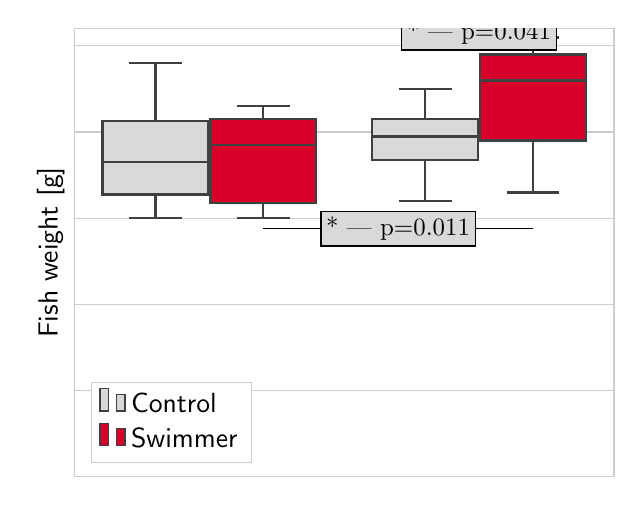
\begin{tikzpicture}

\definecolor{color0}{rgb}{0.83921568627451,0,0.168627450980392}

\begin{axis}[
axis line style={white!80.0!black},
legend cell align={left},
legend style={at={(0.03,0.03)}, anchor=south west, draw=white!80.0!black},
tick align=outside,
x grid style={white!80.0!black},
xmajorticks=false,
xmin=-0.5, xmax=1.5,
xtick style={color=white!15.0!black},
xtick={0,1},
xticklabels={Before Training,After Training},
y grid style={white!80.0!black},
ylabel={Fish weight [g]},
ymajorgrids,
ymajorticks=false,
ymin=0, ymax=0.5205,
ytick style={color=white!15.0!black},
ytick={0,0.1,0.2,0.3,0.4,0.5},
yticklabels={0.0,0.1,0.2,0.3,0.4,0.5}
]
\path [draw=white!25.098039215686274!black, fill=white!85.09803921568627!black, line width=0.9pt]
(axis cs:-0.396,0.3275)
--(axis cs:-0.004,0.3275)
--(axis cs:-0.004,0.4125)
--(axis cs:-0.396,0.4125)
--(axis cs:-0.396,0.3275)
--cycle;
\path [draw=white!25.098039215686274!black, fill=color0, line width=0.9pt]
(axis cs:0.004,0.3175)
--(axis cs:0.396,0.3175)
--(axis cs:0.396,0.415)
--(axis cs:0.004,0.415)
--(axis cs:0.004,0.3175)
--cycle;
\path [draw=white!25.098039215686274!black, fill=white!85.09803921568627!black, line width=0.9pt]
(axis cs:0.604,0.3675)
--(axis cs:0.996,0.3675)
--(axis cs:0.996,0.415)
--(axis cs:0.604,0.415)
--(axis cs:0.604,0.3675)
--cycle;
\path [draw=white!25.098039215686274!black, fill=color0, line width=0.9pt]
(axis cs:1.004,0.39)
--(axis cs:1.396,0.39)
--(axis cs:1.396,0.49)
--(axis cs:1.004,0.49)
--(axis cs:1.004,0.39)
--cycle;
\draw[draw=white!25.098039215686274!black,fill=white!85.09803921568627!black,line width=0.45pt] (axis cs:0,0) rectangle (axis cs:0,0);
\addlegendimage{ybar,ybar legend,draw=white!25.098039215686274!black,fill=white!85.09803921568627!black,line width=0.45pt};
\addlegendentry{Control}

\draw[draw=white!25.098039215686274!black,fill=color0,line width=0.45pt] (axis cs:0,0) rectangle (axis cs:0,0);
\addlegendimage{ybar,ybar legend,draw=white!25.098039215686274!black,fill=color0,line width=0.45pt};
\addlegendentry{Swimmer}

\addplot [line width=0.9pt, white!25.098039215686274!black, forget plot]
table {%
-0.2 0.3275
-0.2 0.3
};
\addplot [line width=0.9pt, white!25.098039215686274!black, forget plot]
table {%
-0.2 0.4125
-0.2 0.48
};
\addplot [line width=0.9pt, white!25.098039215686274!black, forget plot]
table {%
-0.298 0.3
-0.102 0.3
};
\addplot [line width=0.9pt, white!25.098039215686274!black, forget plot]
table {%
-0.298 0.48
-0.102 0.48
};
\addplot [line width=0.9pt, white!25.098039215686274!black, forget plot]
table {%
0.2 0.3175
0.2 0.3
};
\addplot [line width=0.9pt, white!25.098039215686274!black, forget plot]
table {%
0.2 0.415
0.2 0.43
};
\addplot [line width=0.9pt, white!25.098039215686274!black, forget plot]
table {%
0.102 0.3
0.298 0.3
};
\addplot [line width=0.9pt, white!25.098039215686274!black, forget plot]
table {%
0.102 0.43
0.298 0.43
};
\addplot [line width=0.9pt, white!25.098039215686274!black, forget plot]
table {%
0.8 0.3675
0.8 0.32
};
\addplot [line width=0.9pt, white!25.098039215686274!black, forget plot]
table {%
0.8 0.415
0.8 0.45
};
\addplot [line width=0.9pt, white!25.098039215686274!black, forget plot]
table {%
0.702 0.32
0.898 0.32
};
\addplot [line width=0.9pt, white!25.098039215686274!black, forget plot]
table {%
0.702 0.45
0.898 0.45
};
\addplot [line width=0.9pt, white!25.098039215686274!black, forget plot]
table {%
1.2 0.39
1.2 0.33
};
\addplot [line width=0.9pt, white!25.098039215686274!black, forget plot]
table {%
1.2 0.49
1.2 0.51
};
\addplot [line width=0.9pt, white!25.098039215686274!black, forget plot]
table {%
1.102 0.33
1.298 0.33
};
\addplot [line width=0.9pt, white!25.098039215686274!black, forget plot]
table {%
1.102 0.51
1.298 0.51
};
\addplot [line width=0.9pt, white!25.098039215686274!black, forget plot]
table {%
-0.396 0.365
-0.004 0.365
};
\addplot [line width=0.9pt, white!25.098039215686274!black, forget plot]
table {%
0.004 0.385
0.396 0.385
};
\addplot [line width=0.9pt, white!25.098039215686274!black, forget plot]
table {%
0.604 0.395
0.996 0.395
};
\addplot [line width=0.9pt, white!25.098039215686274!black, forget plot]
table {%
1.004 0.46
1.396 0.46
};
\draw[-,black] (axis cs:1.2,0.5151) -- (axis cs:0.8,0.5151);
\draw[] (axis cs:1,0.5151) -- (axis cs:1,0.5151);
\node at (axis cs:1,0.5151)[
  scale=0.9,
  fill=white!85.09803921568627!black,
  draw=black,
  line width=0.6pt,
  inner sep=2.2pt,
  text=black,
  rotate=0.0
]{* | p=0.041};
\draw[-,black] (axis cs:1.2,0.28785) -- (axis cs:0.2,0.28785);
\draw[] (axis cs:0.7,0.28785) -- (axis cs:0.7,0.28785);
\node at (axis cs:0.7,0.28785)[
  scale=0.9,
  fill=white!85.09803921568627!black,
  draw=black,
  line width=0.6pt,
  inner sep=2.2pt,
  text=black,
  rotate=0.0
]{* | p=0.011};
\end{axis}

\end{tikzpicture}
\end{frame}

\note{Length of the fish was measured after anesthesia with procaine from the head to the tail fin (excluding the fin) with a precision of 0.5 mm.}

\begin{frame}
	\frametitle{Endurance}
	% This file was created by matplotlib2tikz v0.7.4.
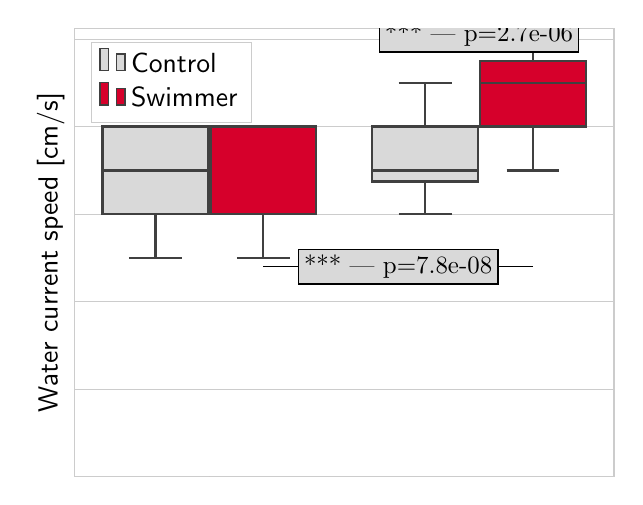
\begin{tikzpicture}

\definecolor{color0}{rgb}{0.83921568627451,0,0.168627450980392}

\begin{axis}[
axis line style={white!80.0!black},
legend cell align={left},
legend style={at={(0.03,0.97)}, anchor=north west, draw=white!80.0!black},
tick align=outside,
x grid style={white!80.0!black},
xmajorticks=false,
xmin=-0.5, xmax=1.5,
xtick style={color=white!15.0!black},
xtick={0,1},
xticklabels={Before Training,After Training},
y grid style={white!80.0!black},
ylabel={Water current speed [cm/s]},
ymajorgrids,
ymajorticks=false,
ymin=0, ymax=51.25,
ytick style={color=white!15.0!black}
]
\path [draw=white!25.098039215686274!black, fill=white!85.09803921568627!black, line width=0.9pt]
(axis cs:-0.396,30)
--(axis cs:-0.004,30)
--(axis cs:-0.004,40)
--(axis cs:-0.396,40)
--(axis cs:-0.396,30)
--cycle;
\path [draw=white!25.098039215686274!black, fill=color0, line width=0.9pt]
(axis cs:0.004,30)
--(axis cs:0.396,30)
--(axis cs:0.396,40)
--(axis cs:0.004,40)
--(axis cs:0.004,30)
--cycle;
\path [draw=white!25.098039215686274!black, fill=white!85.09803921568627!black, line width=0.9pt]
(axis cs:0.604,33.75)
--(axis cs:0.996,33.75)
--(axis cs:0.996,40)
--(axis cs:0.604,40)
--(axis cs:0.604,33.75)
--cycle;
\path [draw=white!25.098039215686274!black, fill=color0, line width=0.9pt]
(axis cs:1.004,40)
--(axis cs:1.396,40)
--(axis cs:1.396,47.5)
--(axis cs:1.004,47.5)
--(axis cs:1.004,40)
--cycle;
\draw[draw=white!25.098039215686274!black,fill=white!85.09803921568627!black,line width=0.45pt] (axis cs:0,0) rectangle (axis cs:0,0);
\addlegendimage{ybar,ybar legend,draw=white!25.098039215686274!black,fill=white!85.09803921568627!black,line width=0.45pt};
\addlegendentry{Control}

\draw[draw=white!25.098039215686274!black,fill=color0,line width=0.45pt] (axis cs:0,0) rectangle (axis cs:0,0);
\addlegendimage{ybar,ybar legend,draw=white!25.098039215686274!black,fill=color0,line width=0.45pt};
\addlegendentry{Swimmer}

\addplot [line width=0.9pt, white!25.098039215686274!black, forget plot]
table {%
-0.2 30
-0.2 25
};
\addplot [line width=0.9pt, white!25.098039215686274!black, forget plot]
table {%
-0.2 40
-0.2 40
};
\addplot [line width=0.9pt, white!25.098039215686274!black, forget plot]
table {%
-0.298 25
-0.102 25
};
\addplot [line width=0.9pt, white!25.098039215686274!black, forget plot]
table {%
-0.298 40
-0.102 40
};
\addplot [line width=0.9pt, white!25.098039215686274!black, forget plot]
table {%
0.2 30
0.2 25
};
\addplot [line width=0.9pt, white!25.098039215686274!black, forget plot]
table {%
0.2 40
0.2 40
};
\addplot [line width=0.9pt, white!25.098039215686274!black, forget plot]
table {%
0.102 25
0.298 25
};
\addplot [line width=0.9pt, white!25.098039215686274!black, forget plot]
table {%
0.102 40
0.298 40
};
\addplot [line width=0.9pt, white!25.098039215686274!black, forget plot]
table {%
0.8 33.75
0.8 30
};
\addplot [line width=0.9pt, white!25.098039215686274!black, forget plot]
table {%
0.8 40
0.8 45
};
\addplot [line width=0.9pt, white!25.098039215686274!black, forget plot]
table {%
0.702 30
0.898 30
};
\addplot [line width=0.9pt, white!25.098039215686274!black, forget plot]
table {%
0.702 45
0.898 45
};
\addplot [line width=0.9pt, white!25.098039215686274!black, forget plot]
table {%
1.2 40
1.2 35
};
\addplot [line width=0.9pt, white!25.098039215686274!black, forget plot]
table {%
1.2 47.5
1.2 50
};
\addplot [line width=0.9pt, white!25.098039215686274!black, forget plot]
table {%
1.102 35
1.298 35
};
\addplot [line width=0.9pt, white!25.098039215686274!black, forget plot]
table {%
1.102 50
1.298 50
};
\addplot [line width=0.9pt, white!25.098039215686274!black, forget plot]
table {%
-0.396 35
-0.004 35
};
\addplot [line width=0.9pt, white!25.098039215686274!black, forget plot]
table {%
0.004 30
0.396 30
};
\addplot [line width=0.9pt, white!25.098039215686274!black, forget plot]
table {%
0.604 35
0.996 35
};
\addplot [line width=0.9pt, white!25.098039215686274!black, forget plot]
table {%
1.004 45
1.396 45
};
\draw[-,black] (axis cs:1.2,50.5) -- (axis cs:0.8,50.5);
\draw[] (axis cs:1,50.5) -- (axis cs:1,50.5);
\node at (axis cs:1,50.5)[
  scale=0.9,
  fill=white!85.09803921568627!black,
  draw=black,
  line width=0.6pt,
  inner sep=2.2pt,
  text=black,
  rotate=0.0
]{*** | p=2.7e-06};
\draw[-,black] (axis cs:1.2,23.9875) -- (axis cs:0.2,23.9875);
\draw[] (axis cs:0.7,23.9875) -- (axis cs:0.7,23.9875);
\node at (axis cs:0.7,23.9875)[
  scale=0.9,
  fill=white!85.09803921568627!black,
  draw=black,
  line width=0.6pt,
  inner sep=2.2pt,
  text=black,
  rotate=0.0
]{*** | p=7.8e-08};
\end{axis}

\end{tikzpicture}
\end{frame}

\begin{frame}
	\frametitle{Gill structure}
	% This file was created by matplotlib2tikz v0.7.4.
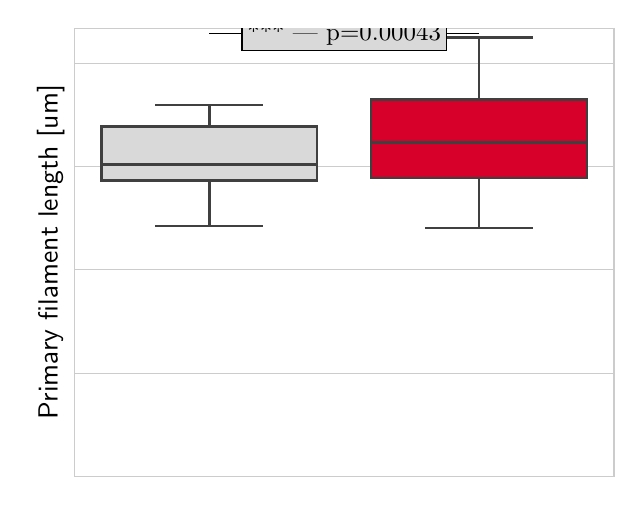
\begin{tikzpicture}

\definecolor{color0}{rgb}{0.83921568627451,0,0.168627450980392}

\begin{axis}[
axis line style={white!80.0!black},
tick align=outside,
x grid style={white!80.0!black},
xmajorticks=false,
xmin=-0.5, xmax=1.5,
xtick style={color=white!15.0!black},
xtick={0,1},
xticklabels={Control,Swimmer},
y grid style={white!80.0!black},
ylabel={Primary filament length [um]},
ymajorgrids,
ymajorticks=false,
ymin=0, ymax=2169.575,
ytick style={color=white!15.0!black}
]
\path [draw=white!25.098039215686274!black, fill=white!85.09803921568627!black, line width=0.9pt]
(axis cs:-0.4,1432.08333333333)
--(axis cs:0.4,1432.08333333333)
--(axis cs:0.4,1693.66666666667)
--(axis cs:-0.4,1693.66666666667)
--(axis cs:-0.4,1432.08333333333)
--cycle;
\path [draw=white!25.098039215686274!black, fill=color0, line width=0.9pt]
(axis cs:0.6,1445.20833333333)
--(axis cs:1.4,1445.20833333333)
--(axis cs:1.4,1824.41666666667)
--(axis cs:0.6,1824.41666666667)
--(axis cs:0.6,1445.20833333333)
--cycle;
\addplot [line width=0.9pt, white!25.098039215686274!black]
table {%
0 1432.08333333333
0 1211.66666666667
};
\addplot [line width=0.9pt, white!25.098039215686274!black]
table {%
0 1693.66666666667
0 1798.33333333333
};
\addplot [line width=0.9pt, white!25.098039215686274!black]
table {%
-0.2 1211.66666666667
0.2 1211.66666666667
};
\addplot [line width=0.9pt, white!25.098039215686274!black]
table {%
-0.2 1798.33333333333
0.2 1798.33333333333
};
\addplot [line width=0.9pt, white!25.098039215686274!black]
table {%
1 1445.20833333333
1 1202
};
\addplot [line width=0.9pt, white!25.098039215686274!black]
table {%
1 1824.41666666667
1 2123.5
};
\addplot [line width=0.9pt, white!25.098039215686274!black]
table {%
0.8 1202
1.2 1202
};
\addplot [line width=0.9pt, white!25.098039215686274!black]
table {%
0.8 2123.5
1.2 2123.5
};
\addplot [line width=0.9pt, white!25.098039215686274!black]
table {%
-0.4 1509.66666666667
0.4 1509.66666666667
};
\addplot [line width=0.9pt, white!25.098039215686274!black]
table {%
0.6 1617.5
1.4 1617.5
};
\draw[-,black] (axis cs:1,2144.735) -- (axis cs:0,2144.735);
\draw[] (axis cs:0.5,2144.735) -- (axis cs:0.5,2144.735);
\node at (axis cs:0.5,2144.735)[
  scale=0.9,
  fill=white!85.09803921568627!black,
  draw=black,
  line width=0.6pt,
  inner sep=2.2pt,
  text=black,
  rotate=0.0
]{*** | p=0.00043};
\end{axis}

\end{tikzpicture}
\end{frame}

\begin{frame}
	\frametitle{Gill volume}
	\only<1>{%
		\pgfmathsetlength{\imagewidth}{0.4\linewidth}%
		\pgfmathsetlength{\imagescale}{\imagewidth/2524}%
		\def\x{1560}% scalebar-x starting at golden ratio of image width of 2524px = 1560
		\def\y{2272}% scalebar-y at 90% of image height of 2524px = 2272
		\def\shadow{4}% shadow parameter for scalebar		
		\begin{tikzpicture}[x=\imagescale,y=-\imagescale]
			\node[anchor=north west, inner sep=0pt, outer sep=0pt] at (0,0) {\includegraphics[width=\imagewidth]{./img/{{Control03_rec00001865}}}};
			% 2524px = 4.1874422mm > 100px = 166um > 301px = 500um, 60px = 100um
			\draw[|-|,blue,thick] (0,1262) -- (2524,1262) node [sloped,midway,above,fill=white,semitransparent,text opacity=1] {\SI{4.1874422}{\milli\meter} (2524px) TEMPORARY!};
			\draw[|-|,thick] (\x+\shadow,\y+\shadow) -- (\x+301+\shadow,\y+\shadow) node [midway,above] {\SI{500}{\micro\meter}};
			\draw[|-|,white,thick] (\x,\y) -- (\x+301,\y) node [midway,above] {\SI{500}{\micro\meter}};
		\end{tikzpicture}%
	}%
	\pgfmathsetlength{\imagewidth}{0.618\linewidth}%
	\pgfmathsetlength{\imagescale}{\imagewidth/2163}%
	\def\x{1337}% scalebar-x starting at golden ratio of image width of 2163px = 1337
	\def\y{1191}% scalebar-y at 90% of image height of 1323px = 1191
	\def\shadow{4}% shadow parameter for scalebar
	\only<2>{%
		\begin{tikzpicture}[x=\imagescale,y=-\imagescale]
			\node[anchor=north west, inner sep=0pt, outer sep=0pt] at (0,0) {\includegraphics[width=\imagewidth]{./img/{{Control03_rec00001865.crop}}}};
			% 2163px = 3.5885251499999997mm > 100px = 166um > 301px = 500um, 60px = 100um
			\draw[|-|,thick] (\x+\shadow,\y+\shadow) -- (\x+301+\shadow,\y+\shadow) node [midway,above] {\SI{500}{\micro\meter}};
			\draw[|-|,white,thick] (\x,\y) -- (\x+301,\y) node [midway,above] {\SI{500}{\micro\meter}};
		\end{tikzpicture}%
		}%
	\only<3>{%
		\begin{tikzpicture}[x=\imagescale,y=-\imagescale]
			\node[anchor=north west, inner sep=0pt, outer sep=0pt] at (0,0) {\includegraphics[width=\imagewidth]{./img/{{control03_rec0000_voi_1865.crop}}}};
			\draw[|-|,thick] (\x+\shadow,\y+\shadow) -- (\x+301+\shadow,\y+\shadow) node [midway,above] {\SI{500}{\micro\meter}};
			\draw[|-|,white,thick] (\x,\y) -- (\x+301,\y) node [midway,above] {\SI{500}{\micro\meter}};
		\end{tikzpicture}%
		}%
	\only<4>{%
		\begin{tikzpicture}[x=\imagescale,y=-\imagescale]
			\node[anchor=north west, inner sep=0pt, outer sep=0pt] at (0,0) {\includegraphics[width=\imagewidth]{./img/{{Control03_thresholded_1500.crop}}}};
			\draw[|-|,thick] (\x+\shadow,\y+\shadow) -- (\x+301+\shadow,\y+\shadow) node [midway,above] {\SI{500}{\micro\meter}};
			\draw[|-|,white,thick] (\x,\y) -- (\x+301,\y) node [midway,above] {\SI{500}{\micro\meter}};
		\end{tikzpicture}%
		}%		
	\includegraphics<4>[height=\textheight]{./img/Control03_thresholded_1500}
	\only<5>{% This file was created by matplotlib2tikz v0.7.4.
\begin{tikzpicture}

%\definecolor{ubRed}{rgb}{0.83921568627451,0,0.168627450980392}

\begin{axis}[
%axis line style={white!80.0!black},
%tick align=outside,
%x grid style={white!80.0!black},
%xmajorticks=false,
xmin=-0.5, xmax=1.5,
%xtick style={color=white!15.0!black},
xtick={0,1},
xticklabels={Control,Swimmer},
%y grid style={white!80.0!black},
ylabel={Gill volume [\si{\micro\litre}]},
%ymajorgrids,
%ymajorticks=false,
ymin=0, %ymax=0.770697055458566,
%ytick style={color=white!15.0!black},
ytick={0,0.1,0.2,0.3,0.4,0.5,0.6,0.7},
yticklabels={0.0,0.1,0.2,0.3,0.4,0.5,0.6,0.7}
]
\path [draw=black, fill=ubGrey]
(axis cs:-0.4,0.447649695726768)
--(axis cs:0.4,0.447649695726768)
--(axis cs:0.4,0.554668101627052)
--(axis cs:-0.4,0.554668101627052)
--(axis cs:-0.4,0.447649695726768)
--cycle;
\path [draw=black, fill=ubRed]
(axis cs:0.6,0.486075630595014)
--(axis cs:1.4,0.486075630595014)
--(axis cs:1.4,0.58742018834191)
--(axis cs:0.6,0.58742018834191)
--(axis cs:0.6,0.486075630595014)
--cycle;
\addplot [line width=0.9pt, green]
table {%
0 0.447649695726768
0 0.376938425845528
};
\addplot [line width=0.9pt, green]
table {%
0 0.554668101627052
0 0.572242192769256
};
\addplot [line width=0.9pt, green]
table {%
-0.2 0.376938425845528
0.2 0.376938425845528
};
\addplot [line width=0.9pt, green]
table {%
-0.2 0.572242192769256
0.2 0.572242192769256
};
\addplot [line width=0.9pt, green]
table {%
1 0.486075630595014
1 0.427215702498488
};
\addplot [line width=0.9pt, green]
table {%
1 0.58742018834191
1 0.623046643313328
};
\addplot [line width=0.9pt, green]
table {%
0.8 0.427215702498488
1.2 0.427215702498488
};
\addplot [line width=0.9pt, green]
table {%
0.8 0.623046643313328
1.2 0.623046643313328
};
%\addplot [black, mark=x, mark size=2, mark options={solid,fill=white!25.098039215686274!black}, only marks]
%table {%
%1 0.749298475419024
%};
\addplot [line width=0.9pt, green]
table {%
-0.4 0.48488362116854
0.4 0.48488362116854
};
\addplot [line width=0.9pt, green]
table {%
0.6 0.542154490975104
1.4 0.542154490975104
};
\addplot [only marks, draw=black, fill=ubGrey, colormap/blackwhite]
table{%
x                      y
-0.177324872476305 0.572242192769256
-0.063553536460232 0.471672297437017
-0.127173503667371 0.56475262570696
-0.140536340773334 0.568003444252336
-0.0449978015031713 0.524414529387328
0.0399882813308409 0.484753900995424
-0.0758154144069236 0.376938425845528
-0.0334201811304397 0.439642161823352
-0.0234274539581418 0.41752174920648
0.118939057427129 0.485013341341656
};
\addplot [only marks, draw=black, fill=ubRed, colormap/blackwhite]
table{%
x                      y
0.968335974120825 0.567564796770337
1.07007525219083 0.503736968660552
0.991193737838358 0.449384355640976
0.886410654649808 0.480188517906501
1.08845905619196 0.623046643313328
0.85356807648219 0.577596442831624
1.17491726910287 0.590694770178672
1.16555444601312 0.516744185179872
1.00788018410688 0.749298475419024
1.09781093186924 0.427215702498488
};
\draw[|-|] (axis cs:1,0.756791460173214) -- (axis cs:0,0.756791460173214) node [midway,above] {};
\draw[] (axis cs:0.5,0.756791460173214) -- (axis cs:0.5,0.756791460173214);
\node at (axis cs:0.5,0.756791460173214)[
  scale=0.9,
  fill=ubGrey,
  draw=black,
  line width=0.6pt,
  inner sep=2.2pt,
  text=black,
  rotate=0.0
]{* | p=0.048};
\end{axis}

\end{tikzpicture}}
\end{frame}

\begin{frame}
	\frametitle{Gill complexity}
	\begin{tikzpicture}[remember picture,overlay]%
		\node[xshift=0,yshift=-0.085\paperheight-0.016\paperheight/2] at (current page.center){%
			\animategraphics[palindrome,autoplay,width=\paperwidth,every=\everyframe]{25}{./mov/complexity/control03_thresholded_0}{025}{256}%
			};%
	\end{tikzpicture}%
\end{frame}

\begin{frame}
	\frametitle{Gill complexity}
	\pgfmathsetlength{\imagewidth}{0.618\linewidth}%
	\pgfmathsetlength{\imagescale}{\imagewidth/2163}%
	\def\x{1337}% scalebar-x starting at golden ratio of image width of 2163px = 1337
	\def\y{1191}% scalebar-y at 90% of image height of 1323px = 1191
	\def\shadow{4}% shadow parameter for scalebar	
	\only<1>{%
		\begin{tikzpicture}[x=\imagescale,y=-\imagescale]
			\node[anchor=north west, inner sep=0pt, outer sep=0pt] at (0,0) {\includegraphics[width=\imagewidth]{./img/{{Control03_thresholded_1500.crop}}}};
			\draw[|-|,thick] (\x+\shadow,\y+\shadow) -- (\x+301+\shadow,\y+\shadow) node [midway,above] {\SI{500}{\micro\meter}};
			\draw[|-|,white,thick] (\x,\y) -- (\x+301,\y) node [midway,above] {\SI{500}{\micro\meter}};
		\end{tikzpicture}%
		}%		
	\only<2>{%
		\begin{tikzpicture}[x=\imagescale,y=-\imagescale]
			\node[anchor=north west, inner sep=0pt, outer sep=0pt] at (0,0) {\includegraphics[width=\imagewidth]{./img/{{Control03_area_organ_1500.crop.edit}}}};
			\draw[|-|,thick] (\x+\shadow,\y+\shadow) -- (\x+301+\shadow,\y+\shadow) node [midway,above] {\SI{500}{\micro\meter}};
			\draw[|-|,white,thick] (\x,\y) -- (\x+301,\y) node [midway,above] {\SI{500}{\micro\meter}};
		\end{tikzpicture}%
		}%		
	\only<3>{%
		\begin{tikzpicture}[x=\imagescale,y=-\imagescale]
			\node[anchor=north west, inner sep=0pt, outer sep=0pt] at (0,0) {\includegraphics[width=\imagewidth]{./img/{{Control03_area_organ_1500.crop.combination}}}};
			\draw[|-|,thick] (\x+\shadow,\y+\shadow) -- (\x+301+\shadow,\y+\shadow) node {\SI{500}{\micro\meter}};
			\draw[|-|,white,thick] (\x,\y) -- (\x+301,\y) node [midway,above] {\SI{500}{\micro\meter}};
		\end{tikzpicture}%
		}%		
	\only<4>{% This file was created by matplotlib2tikz v0.7.4.
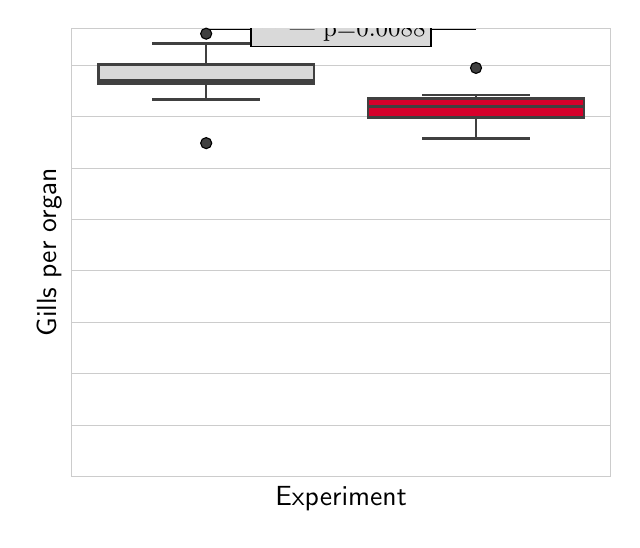
\begin{tikzpicture}

\definecolor{color0}{rgb}{0.83921568627451,0,0.168627450980392}

\begin{axis}[
axis line style={white!80.0!black},
tick align=outside,
x grid style={white!80.0!black},
xlabel={Experiment},
xmajorticks=false,
xmin=-0.5, xmax=1.5,
xtick style={color=white!15.0!black},
xtick={0,1},
xticklabels={Control,Swimmer},
y grid style={white!80.0!black},
ylabel={Gills per organ},
ymajorgrids,
ymajorticks=false,
ymin=0, ymax=0.436126551884328,
ytick style={color=white!15.0!black},
ytick={0,0.05,0.1,0.15,0.2,0.25,0.3,0.35,0.4},
yticklabels={0.00,0.05,0.10,0.15,0.20,0.25,0.30,0.35,0.40}
]
\path [draw=white!25.098039215686274!black, fill=white!85.09803921568627!black, line width=0.9pt]
(axis cs:-0.4,0.382496841309432)
--(axis cs:0.4,0.382496841309432)
--(axis cs:0.4,0.40078453974052)
--(axis cs:-0.4,0.40078453974052)
--(axis cs:-0.4,0.382496841309432)
--cycle;
\path [draw=white!25.098039215686274!black, fill=color0, line width=0.9pt]
(axis cs:0.6,0.349508101341073)
--(axis cs:1.4,0.349508101341073)
--(axis cs:1.4,0.367828846032819)
--(axis cs:0.6,0.367828846032819)
--(axis cs:0.6,0.349508101341073)
--cycle;
\addplot [line width=0.9pt, white!25.098039215686274!black]
table {%
0 0.382496841309432
0 0.366846367137451
};
\addplot [line width=0.9pt, white!25.098039215686274!black]
table {%
0 0.40078453974052
0 0.421306108182572
};
\addplot [line width=0.9pt, white!25.098039215686274!black]
table {%
-0.2 0.366846367137451
0.2 0.366846367137451
};
\addplot [line width=0.9pt, white!25.098039215686274!black]
table {%
-0.2 0.421306108182572
0.2 0.421306108182572
};
\addplot [black, mark=*, mark size=2, mark options={solid,fill=white!25.098039215686274!black}, only marks]
table {%
0 0.324346236114214
0 0.430803679704798
};
\addplot [line width=0.9pt, white!25.098039215686274!black]
table {%
1 0.349508101341073
1 0.328636765492142
};
\addplot [line width=0.9pt, white!25.098039215686274!black]
table {%
1 0.367828846032819
1 0.370980682541585
};
\addplot [line width=0.9pt, white!25.098039215686274!black]
table {%
0.8 0.328636765492142
1.2 0.328636765492142
};
\addplot [line width=0.9pt, white!25.098039215686274!black]
table {%
0.8 0.370980682541585
1.2 0.370980682541585
};
\addplot [black, mark=*, mark size=2, mark options={solid,fill=white!25.098039215686274!black}, only marks]
table {%
1 0.397507730617411
};
\addplot [line width=0.9pt, white!25.098039215686274!black]
table {%
-0.4 0.385498429400225
0.4 0.385498429400225
};
\addplot [line width=0.9pt, white!25.098039215686274!black]
table {%
0.6 0.359924925696058
1.4 0.359924925696058
};
\draw[-,black] (axis cs:1,0.435111716501846) -- (axis cs:0,0.435111716501846);
\draw[] (axis cs:0.5,0.435111716501846) -- (axis cs:0.5,0.435111716501846);
\node at (axis cs:0.5,0.435111716501846)[
  scale=0.9,
  fill=white!85.09803921568627!black,
  draw=black,
  line width=0.6pt,
  inner sep=2.2pt,
  text=black,
  rotate=0.0
]{** | p=0.0088};
\end{axis}

\end{tikzpicture}}
\end{frame}

\begin{frame}[label=current]
	\frametitle{\ce{O2} consumption}
	% This file was created by matplotlib2tikz v0.7.4.
\begin{tikzpicture}

%\definecolor{ubRed}{rgb}{0.83921568627451,0,0.168627450980392}

\begin{axis}[
%axis line style={white!80.0!black},
%legend cell align={left},
%legend style={draw=white!80.0!black},
%tick align=outside,
%x grid style={white!80.0!black},
%xmajorticks=false,
xmin=-0.5, xmax=1.5,
%xtick style={color=white!15.0!black},
xtick={0,1},
xticklabels={Before Training,After Training},
%y grid style={white!80.0!black},
ylabel={Normalized \ce{O2}-consumption},
%ymajorgrids,
%ymajorticks=false,
ymin=0, %ymax=0.0596151429433558,
%ytick style={color=white!15.0!black}
]
\path [draw=black, fill=ubGrey]
(axis cs:-0.396,0.0250714285714286)
--(axis cs:-0.004,0.0250714285714286)
--(axis cs:-0.004,0.0422142857142857)
--(axis cs:-0.396,0.0422142857142857)
--(axis cs:-0.396,0.0250714285714286)
--cycle;
\path [draw=black, fill=ubRed]
(axis cs:0.004,0.0261494252873564)
--(axis cs:0.396,0.0261494252873564)
--(axis cs:0.396,0.0355862068965518)
--(axis cs:0.004,0.0355862068965518)
--(axis cs:0.004,0.0261494252873564)
--cycle;
\path [draw=black, fill=ubGrey]
(axis cs:0.604,0.0207167070217918)
--(axis cs:0.996,0.0207167070217918)
--(axis cs:0.996,0.0310344827586207)
--(axis cs:0.604,0.0310344827586207)
--(axis cs:0.604,0.0207167070217918)
--cycle;
\path [draw=black, fill=ubRed]
(axis cs:1.004,0.0314)
--(axis cs:1.396,0.0314)
--(axis cs:1.396,0.0353793103448276)
--(axis cs:1.004,0.0353793103448276)
--(axis cs:1.004,0.0314)
--cycle;
\addplot [only marks, draw=black, fill=ubGrey, colormap/blackwhite]
table{%
x                      y
};
%\addlegendentry{Control}
\addplot [only marks, draw=ubRed, fill=ubRed, colormap/blackwhite]
table{%
x                      y
};
%\addlegendentry{Swimmer}
\draw[draw=black,fill=ubGrey,line width=0.45pt] (axis cs:0,0) rectangle (axis cs:0,0);
\addlegendimage{ybar,ybar legend,draw=black,fill=ubGrey,line width=0.45pt};
%\addlegendentry{Control}

\draw[draw=black,fill=ubRed,line width=0.45pt] (axis cs:0,0) rectangle (axis cs:0,0);
\addlegendimage{ybar,ybar legend,draw=black,fill=ubRed,line width=0.45pt};
%\addlegendentry{Swimmer}

\addplot [forget plot]
table {%
-0.2 0.0250714285714286
-0.2 0.0204
};
\addplot [forget plot]
table {%
-0.2 0.0422142857142857
-0.2 0.0573103448275862
};
\addplot [forget plot]
table {%
-0.298 0.0204
-0.102 0.0204
};
\addplot [forget plot]
table {%
-0.298 0.0573103448275862
-0.102 0.0573103448275862
};
\addplot [forget plot]
table {%
0.2 0.0261494252873564
0.2 0.0231724137931034
};
\addplot [forget plot]
table {%
0.2 0.0355862068965518
0.2 0.037448275862069
};
\addplot [forget plot]
table {%
0.102 0.0231724137931034
0.298 0.0231724137931034
};
\addplot [forget plot]
table {%
0.102 0.037448275862069
0.298 0.037448275862069
};
%\addplot [black, mark=x, mark size=2, mark options={solid,fill=white!25.098039215686274!black}, only marks, forget plot]
%table {%
%0.2 0.0555
%0.2 0.0520714285714286
%};
\addplot [forget plot]
table {%
0.8 0.0207167070217918
0.8 0.0171724137931034
};
\addplot [forget plot]
table {%
0.8 0.0310344827586207
0.8 0.0406315789473684
};
\addplot [forget plot]
table {%
0.702 0.0171724137931034
0.898 0.0171724137931034
};
\addplot [forget plot]
table {%
0.702 0.0406315789473684
0.898 0.0406315789473684
};
\addplot [forget plot]
table {%
1.2 0.0314
1.2 0.0295862068965517
};
\addplot [forget plot]
table {%
1.2 0.0353793103448276
1.2 0.0389508196721311
};
\addplot [forget plot]
table {%
1.102 0.0295862068965517
1.298 0.0295862068965517
};
\addplot [forget plot]
table {%
1.102 0.0389508196721311
1.298 0.0389508196721311
};
%\addplot [black, mark=x, mark size=2, mark options={solid,fill=white!25.098039215686274!black}, only marks, forget plot]
%table {%
%1.2 0.0443571428571429
%};
\addplot [forget plot]
table {%
-0.396 0.0314188034188034
-0.004 0.0314188034188034
};
\addplot [forget plot]
table {%
0.004 0.0288049450549451
0.396 0.0288049450549451
};
\addplot [forget plot]
table {%
0.604 0.0248307692307692
0.996 0.0248307692307692
};
\addplot [forget plot]
table {%
1.004 0.0335555555555556
1.396 0.0335555555555556
};
\addplot [only marks, draw=black, fill=ubGrey, colormap/blackwhite, forget plot]
table{%
x                      y
-0.109684927076163 0.0573103448275862
-0.162222170659982 0.0204
-0.137899343546467 0.0351428571428571
-0.198167488856793 0.0213333333333333
-0.147249059859333 0.0248571428571429
-0.235512167697188 0.0286153846153846
-0.291106410161967 0.0526
-0.176918493117764 0.0445714285714286
-0.267179267616746 0.0257142857142857
-0.161496334832033 0.0342222222222222
};
\addplot [only marks, draw=black, fill=ubRed, colormap/blackwhite, forget plot]
table{%
x                      y
0.186047985821138 0.0280714285714286
0.216134773621717 0.037448275862069
0.278043845731273 0.0231724137931034
0.259995026157038 0.0279310344827586
0.185715158092205 0.0248571428571429
0.233976093639374 0.0555
0.224580748387237 0.03
0.135163802218661 0.0520714285714286
0.247404466948641 0.0295384615384615
0.124127520955504 0.0255555555555556
};
\addplot [only marks, draw=black, fill=ubGrey, colormap/blackwhite, forget plot]
table{%
x                      y
0.783157291530245 0.0282
0.816453883089452 0.0211525423728814
0.842741800235094 0.0171724137931034
0.827774123907361 0.0291724137931034
0.763178518080526 0.0214615384615385
0.861346805851937 0.0184285714285714
0.867557847909687 0.0205714285714286
0.841898745896218 0.034551724137931
0.867821475134066 0.0316551724137931
0.815262520218799 0.0406315789473684
};
\addplot [only marks, draw=black, fill=ubRed, colormap/blackwhite, forget plot]
table{%
x                      y
1.13965655089032 0.0389508196721311
1.19963128305166 0.03
1.14390319114155 0.0316190476190476
1.26572870566399 0.0295862068965517
1.2560502561859 0.0335555555555556
1.26314712848455 0.0338
1.20557979517041 0.0443571428571429
1.28576648725987 0.0314
1.13674718647357 0.0353793103448276
};
\draw[|-|] (axis cs:1.2,0.0578834482758621) -- (axis cs:0.8,0.0578834482758621) node [midway,above] {};
\draw[] (axis cs:1,0.0578834482758621) -- (axis cs:1,0.0578834482758621);
\node at (axis cs:1,0.0578834482758621)[
  scale=0.9,
  fill=ubGrey,
  draw=black,
  line width=0.6pt,
  inner sep=2.2pt,
  text=black,
  rotate=0.0
]{** | p=0.0081};
\end{axis}

\end{tikzpicture}
\end{frame}

\begin{frame}[label=current]
	\frametitle{Wee!}
	\begin{itemize}
		\item The zebrafish respiratory organ has a high plasticity
		\item After endurance training respiratory organ is larger and more airy, facilitating \ce{O2} uptake.
		\item Increase in critical speed, body weight and body length
		\item Increase in oxygen consumption of trained zebrafish
		\item Morphological differences in gills
		\item Longer primary filaments and more secondary filaments
		\item Increase of total gill volume
		\pause
		\item \emph{Adaptation of the respiratory organ to endurance training has been showed for the first time}
	\end{itemize}
\end{frame}

\begin{frame}[label=current]
	\frametitle{Thanks!}
	\begin{columns}
		\begin{column}{0.618\linewidth}
		\begin{itemize}
			\item<1-> Team from the \emph{Topographic and clinical Anatomy} group
			\begin{itemize}
				\item<1-> Dea Aaldijk, Matthias Messerli
				\item<1-> Ruslan Hlushchuk, Valentin Djonov
				\item<1-> Fluri A.\ M.\ Wieland, Oleksiy Khoma
				\item<1-> Sarya Fark, Helena Röss
			\end{itemize}
			\item<1-> Other important people at the Institute of Anatomy
			\begin{itemize}
				\item<1-> Werner Graber, Jeannine Wagner-Zimmermann and Beat Haenni
				\item<1-> Regula Buergy, Eveline Yao and Sara Soltermann
				\item<1-> Marcos Sande, Carolina Garcia
				\item<1-> Ines Marquez, Xavier Langa and Alexander Uwe Ernst
			\end{itemize}
			\item<1-> SNF
			\item<2-> You, for listening
			\item<3-> Questions?
		\end{itemize}
		\end{column}
		\begin{column}{0.382\linewidth}
			\includegraphics<1->[width=\linewidth]{./img/team}
		\end{column}
	\end{columns}
\end{frame}

\begin{frame}
	\frametitle{References}
	\renewcommand*{\bibfont}{\footnotesize}
	% No parentheses around the (empty) year: https://tex.stackexchange.com/a/147537
	%\renewcommand{\bibopenparen}{\addcomma\addspace}
	%\renewcommand{\bibcloseparen}{\addcomma\addspace}
	\setbeamertemplate{bibliography item}{\insertbiblabel}
	\printbibliography
\end{frame}

\begin{frame}
	\frametitle{Colophon}
	\begin{itemize}
			\item \href{https://github.com/habi/20190605_BrukerUserMeeting}{The \LaTeX source of this \textsc{beamer} presentation is available on GitHub.}
		\item \href{https://github.com/habi/Zebra-Fish-Gills/}{The full analysis of the data (in \faPython) is also available on GitHub}
		\item \href{http://intern.unibe.ch/dienstleistungen/corporate_design_und_vorlagen/praesentationen/index_ger.html}{The presentation template is from \emph{Corporate Design und Vorlagen, University of Bern}}
	\end{itemize}
\end{frame}

\end{document}
